\chapter{Studi Literatur}
\label{chapter:studi-literatur}

Pada bab ini, akan diisi oleh studi literatur, hal-hal yang berkaitan dengan topik persoalan tugas akhir akan dipaparkan dalam bab ini guna untuk memberikan informasi mengenai dasar teori dan studi yang dipakai. Bab ini diharapkan membantu pembaca untuk mengerti dalam membaca penelitian tugas akhir ini.


\section{\textit{Service}}

\textit{Service} dapat diartikan sebagai sebuah teknologi atau cara kerja yang dapat digunakan untuk memberikan keuntungan ataupun menyelesaikan suatu pekerjaan. Selain itu \textit{service} juga dapat diartikan sebagai abstraksi dari sebuah proses bisnis. \parencite{osullivan2002}

Secara umum \textit{Service} Memiliki tiga fitur utama yaitu.
\begin{enumerate}
  \item \textit{Service} dapat melakukan sebuah aksi atau pekerjaan untuk orang lain,
  \item \textit{Service} adalah sebuah aset yang memiliki sebuah nilai yang dapat diturunkan dari penyedia ke pengguna,
  \item \textit{Service} dapat di bungkus pada service lainnya (sub-services),
\end{enumerate}

Untuk menggabungkan \textit{service}, terdapat dua cara yaitu agregasi dan komposisi. Agregasi memiliki pendekatan untuk menggabungkan dua atau lebih \textit{service} dan membuat satu \textit{entrypoint} untuk seluruh \textit{service} tersebut. Berbeda dengan komposisi, komposisi menggunakan pendekatan untuk mengintegrasikan seluruh sub-\textit{services} yang ada dengan cara membuat jalur komunikasi antar \textit{service} dan setiap \textit{service} memiliki hubungan tertentu dengan \textit{service} lainnya.

Interaksi pada sebuah \textit{service} haruslah minimal memiliki tiga elemen, \textit{service provider}, \textit{service requestor/client}, serta \textit{\textit{service registry}}, namun terdapat juga elemen ke empat pada beberapa kasus yaitu \textit{service broker}. Illustrasi dapat dilhat pada gambar \ref{fig:tiga-elemen-service}

\begin{figure}[ht]
  \centering
  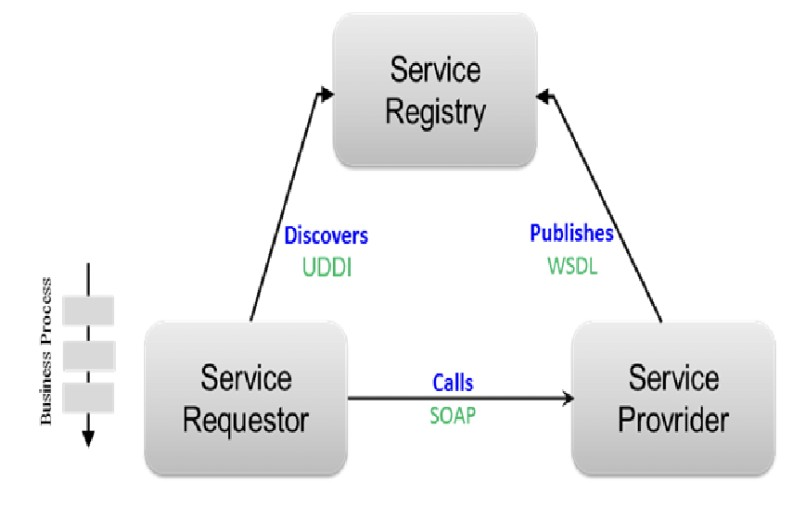
\includegraphics[width=0.8\textwidth]{chapter-2/tiga-elemen-service.jpg}
  \caption{Tiga Elemen pada Interaksi Service, \parencite{abugessaisa2023}}
  \label{fig:tiga-elemen-service}
\end{figure}

\textit{Service requestor} mengirimkan permintaannya serta kebutuhannya kepada \textit{service registry} untuk dicarikan service yang sesuai dengan kebutuhannya. Namun pada beberapa kasus khusus, \textit{service requestor}
sudah memiliki \textquotedblleft contract \textquotedblright dengan \textit{provider} tujuannya sehingga bisa langsung melakukan \textit{request} ke \textit{provider} tanpa bantuan dari \textit{service registry}.

Service \textit{provider} menyediakan \textit{service} yang dapat dikonsumsi oleh publik, agar \textit{service} nya dapat digunakan oleh requestor, \textit{service} \textit{provider} akan memberikan list \textit{services} yang dimiliki kepada registry untuk disimpan pada sebuah \textquotedblleft catalogue \textquotedblright yang dimiliki oleh registry.\textit{Service registry} berperan sebagai penengah dalam komunikasi \textit{requestor} dan \textit{provider}. \textit{Service registry} memiliki \textquotedblleft catalogue \textquotedblright yang menyimpan list berbagai macam \textit{service provider} yang dapat digunakan oleh \textit{service requestor}.

Dengan adanya ketiga elemen tersebut, interaksi pada \textit{services} dapat berjalan sehingga menciptakan suatu fungsionalitas seperti proses bisnis ataupun pemenuhan kebutuhan lainnya.


\section{\textit{Service Mesh}}

\subsection{Definisi}

\textit{Service mesh} adalah sebuah infrastruktur yang memanage \textit{Service} komunikasi antar \textit{service}. \textit{Service mesh} dibuat dengan tujuan untuk memberikan layer tambahan untuk architecture yang dibuat tanpa harus membuat kode aplikasi pada setiap \textit{service} untuk berkomunikasi.\parencite{li2019}

Jika terdapat dua buah \textit{service}, kedua \textit{service} tersebut harus membuat sebuah interface ataupun cara menghubungkan masing masing \textit{service} untuk berkomunikasi karena perlu adanya beberapa penyesuaian, seperti penyesuaian bahasa pemrograman karena mungkin saja kedua \textit{service} tersebut menggunakan bahasa pemrograman yang berbeda.

Setiap \textit{service} juga perlu menyesuaikan cara dari setiap \textit{service} tersebut menerima dan mengirim request. Beberapa \textit{service} mungkin saja menggunakan gRPC untuk menerima dan mengirim request dan \textit{service} lain menggunakan REST ataupun graphQL. Bayangkan jika kita memiliki lebih dari 100 \textit{service} yang ingin ber orkestrasi dan berkomunikasi satu sama lain, kita harus membuat interface untuk setiap \textit{service} yang ada dan hal ini sangat memakan waktu.

\textit{Service mesh} hadir untuk menyelesaikan masalah ini terutama masalah komunikasi internal antar \textit{service}. Selain itu, \textit{Service mesh} juga memberikan fitur seperti \textit{device discovery}, \textit{central authentication}, \textit{access control}, \textit{load balancing}, \textit{logging}, serta \textit{monitoring}. Selain memberikan fitur tersebut, \textit{\textit{service} mesh} juga harus memiliki \textit{reliability} serta \textit{fault tolerance}. \parencite{li2019}

\textit{Service mesh} pada umumnya memiliki dua plane, \textit{control plane} dan \textit{data plane}. \textit{control plane} merupakan sebuah tempat terpusat untuk mengontrol jaringan mulai dari \textit{device discovery}, \textit{logging dan monitoring}, ataupun menjaga \textit{service level agreement} (SLA) agar \textit{availability} dari \textit{service} yang ada memiliki nilai yang baik. \textit{data plane} sering disebut sebagai \textit{forwarding plane} karena bertujuan untuk meneruskan ataupun menerima request dari \textit{service} yang dituju sesuai arahan dari \textit{control plane}. Kedua \textit{plane} ini menjadi komponen paling penting dalam pembuatan \textit{\textit{service} mesh}.

\textit{Service mesh} dapat melakukan beberapa jenis interaksi terhadap komponen kubernetes, interaksi ini merupakan keunggulan \textit{service mesh} untuk mendukung berbagai macam fungsionalitas dan desain arsitektur. Berikut merupakan tujuh jenis interaksi yang dapat dilakukan oleh \textit{service mesh} \parencite{ganguli2021}

\begin{enumerate}
  \item Komunikasi antar \textit{pod}
  \item Komunikasi \textit{pod} dengan \textit{service}
  \item Komunikasi \textit{ingress controller} dengan \textit{pod} dan sebaliknya
  \item Komunikasi \textit{load balancer} dengan \textit{pod} dan sebaliknya
  \item Komunikasi \textit{pod} dengan \textit{egress controller}
  \item \textit{API gateway to service and vice-versa}
  \item \textit{TLS termination}
\end{enumerate}.

Sudah banyak produk ataupun aplikasi yang menawarkan solusi untuk menyelesaikan masalah \textit{\textit{service} Mesh}, diantaranya Istio, Linkerd, Airbnb Synapse, dan AWS App Mesh. Keempat aplikasi tersebut memiliki cara tersendiri agar \textit{\textit{service} mesh} dapat berjalan dengan baik. Berikut tabel perbandingan dari keempat produk tersebut


\begin{longtable}{|p{1.5cm}|p{1.5cm}|p{1.5cm}|p{1.5cm}|p{1.5cm}|p{1.5cm}|p{1.5cm}|}
  \caption{Perbandingan platform solusi \textit{service mesh} \parencite{li2019}} \label{tab:perbandingan-service-mesh}                                                                                                                                \\
  \hline
  \rowcolor{gray!30} \textbf{Aplikasi} & \textbf{\textit{Data plane}} & \textbf{\textit{Open source}} & \textbf{\textit{Activeness}} & \textbf{\textit{Major advantage}}    & \textbf{\textit{Critical limitation}} & \textbf{\textit{Rating overall}} \\
  \hline
  \endfirsthead

  \endhead

  % \textit{Intelligent Workload Factoring for a Hybrid Cloud Computing Model}, \parencite{zhang} & VM & \textit{Request Rate} & Reaktif & ARIMA \tabularnewline
  Istio                                & Envoy                        & Yes                           & Good                         & Growing Community and Fast Iteration & Lack of support                       & Moderate \tabularnewline \hline

  Linkerd2                             & Linkerd-proxy                & Yes                           & Good                         & Stability and CNCF Accepted          & Potential vendor Lock-in              & Good \tabularnewline \hline

  AWS App Mesh                         & Envoy                        & No                            & Good                         & Native Compatibility with AWS        & Closed Ecosystem                      & Preview \tabularnewline \hline

  Airbnb Synapse                       & HAProxy / Nginx              & Yes                           & Poor                         & N/A                                  & Limited Features                      & Poor \tabularnewline \hline

  \hline
\end{longtable}


\subsection{Interaksi}

\textit{Service mesh} dapat melakukan beberapa jenis interaksi terhadap, interaksi ini merupakan keunggulan \textit{service mesh} untuk mendukung berbagai macam fungsionalitas dan desain arsitektur. Berikut merupakan tujuh jenis interaksi yang dapat dilakukan oleh \textit{service mesh} \parencite{ganguli2021}

\begin{enumerate}
  \item Komunikasi antar \textit{pod}
  \item Komunikasi \textit{pod} dengan \textit{service}
  \item Komunikasi \textit{ingress controller} dengan \textit{pod} dan sebaliknya
  \item Komunikasi \textit{load balancer} dengan \textit{pod} dan sebaliknya
  \item Komunikasi \textit{pod} dengan \textit{egress controller}
  \item \textit{API gateway to service and vice-versa}
  \item \textit{TLS termination}
\end{enumerate}

\subsection{Definisi}

\textit{Service mesh} adalah sebuah infrastruktur yang memanage \textit{Service} komunikasi antar \textit{service}. \textit{Service mesh} dibuat dengan tujuan untuk memberikan layer tambahan untuk architecture yang dibuat tanpa harus membuat kode aplikasi pada setiap \textit{service} untuk berkomunikasi.\parencite{li2019}

Jika terdapat dua buah \textit{service}, kedua \textit{service} tersebut harus membuat sebuah interface ataupun cara menghubungkan masing masing \textit{service} untuk berkomunikasi karena perlu adanya beberapa penyesuaian, seperti penyesuaian bahasa pemrograman karena mungkin saja kedua \textit{service} tersebut menggunakan bahasa pemrograman yang berbeda.

Setiap \textit{service} juga perlu menyesuaikan cara dari setiap \textit{service} tersebut menerima dan mengirim request. Beberapa \textit{service} mungkin saja menggunakan gRPC untuk menerima dan mengirim request dan \textit{service} lain menggunakan REST ataupun graphQL. Bayangkan jika kita memiliki lebih dari 100 \textit{service} yang ingin ber orkestrasi dan berkomunikasi satu sama lain, kita harus membuat interface untuk setiap \textit{service} yang ada dan hal ini sangat memakan waktu.

\textit{Service mesh} hadir untuk menyelesaikan masalah ini terutama masalah komunikasi internal antar \textit{service}. Selain itu, \textit{Service mesh} juga memberikan fitur seperti \textit{device discovery}, \textit{central authentication}, \textit{access control}, \textit{load balancing}, \textit{logging}, serta \textit{monitoring}. Selain memberikan fitur tersebut, \textit{\textit{service} mesh} juga harus memiliki \textit{reliability} serta \textit{fault tolerance}. \parencite{li2019}

\textit{Service mesh} pada umumnya memiliki dua plane, \textit{control plane} dan \textit{data plane}. \textit{control plane} merupakan sebuah tempat terpusat untuk mengontrol jaringan mulai dari \textit{device discovery}, \textit{logging dan monitoring}, ataupun menjaga \textit{service level agreement} (SLA) agar \textit{availability} dari \textit{service} yang ada memiliki nilai yang baik. \textit{data plane} sering disebut sebagai \textit{forwarding plane} karena bertujuan untuk meneruskan ataupun menerima request dari \textit{service} yang dituju sesuai arahan dari \textit{control plane}. Kedua \textit{plane} ini menjadi komponen paling penting dalam pembuatan \textit{\textit{service} mesh}.

\textit{Service mesh} dapat melakukan beberapa jenis interaksi terhadap komponen kubernetes, interaksi ini merupakan keunggulan \textit{service mesh} untuk mendukung berbagai macam fungsionalitas dan desain arsitektur. Berikut merupakan tujuh jenis interaksi yang dapat dilakukan oleh \textit{service mesh} \parencite{ganguli2021}

\begin{enumerate}
  \item Komunikasi antar \textit{pod}
  \item Komunikasi \textit{pod} dengan \textit{service}
  \item Komunikasi \textit{ingress controller} dengan \textit{pod} dan sebaliknya
  \item Komunikasi \textit{load balancer} dengan \textit{pod} dan sebaliknya
  \item Komunikasi \textit{pod} dengan \textit{egress controller}
  \item \textit{API gateway to service and vice-versa}
  \item \textit{TLS termination}
\end{enumerate}.

Sudah banyak produk ataupun aplikasi yang menawarkan solusi untuk menyelesaikan masalah \textit{\textit{service} Mesh}, diantaranya Istio, Linkerd, Airbnb Synapse, dan AWS App Mesh. Keempat aplikasi tersebut memiliki cara tersendiri agar \textit{\textit{service} mesh} dapat berjalan dengan baik. Berikut tabel perbandingan dari keempat produk tersebut


\begin{longtable}{|p{1.5cm}|p{1.5cm}|p{1.5cm}|p{1.5cm}|p{1.5cm}|p{1.5cm}|p{1.5cm}|}
  \caption{Perbandingan platform solusi \textit{service mesh} \parencite{li2019}} \label{tab:perbandingan-service-mesh}                                                                                                                                \\
  \hline
  \rowcolor{gray!30} \textbf{Aplikasi} & \textbf{\textit{Data plane}} & \textbf{\textit{Open source}} & \textbf{\textit{Activeness}} & \textbf{\textit{Major advantage}}    & \textbf{\textit{Critical limitation}} & \textbf{\textit{Rating overall}} \\
  \hline
  \endfirsthead

  \endhead

  % \textit{Intelligent Workload Factoring for a Hybrid Cloud Computing Model}, \parencite{zhang} & VM & \textit{Request Rate} & Reaktif & ARIMA \tabularnewline
  Istio                                & Envoy                        & Yes                           & Good                         & Growing Community and Fast Iteration & Lack of support                       & Moderate \tabularnewline \hline

  Linkerd2                             & Linkerd-proxy                & Yes                           & Good                         & Stability and CNCF Accepted          & Potential vendor Lock-in              & Good \tabularnewline \hline

  AWS App Mesh                         & Envoy                        & No                            & Good                         & Native Compatibility with AWS        & Closed Ecosystem                      & Preview \tabularnewline \hline

  Airbnb Synapse                       & HAProxy / Nginx              & Yes                           & Poor                         & N/A                                  & Limited Features                      & Poor \tabularnewline \hline

  \hline
\end{longtable}


\subsection{Interaksi}

\textit{Service mesh} dapat melakukan beberapa jenis interaksi terhadap, interaksi ini merupakan keunggulan \textit{service mesh} untuk mendukung berbagai macam fungsionalitas dan desain arsitektur. Berikut merupakan tujuh jenis interaksi yang dapat dilakukan oleh \textit{service mesh} \parencite{ganguli2021}

\begin{enumerate}
  \item Komunikasi antar \textit{pod}
  \item Komunikasi \textit{pod} dengan \textit{service}
  \item Komunikasi \textit{ingress controller} dengan \textit{pod} dan sebaliknya
  \item Komunikasi \textit{load balancer} dengan \textit{pod} dan sebaliknya
  \item Komunikasi \textit{pod} dengan \textit{egress controller}
  \item \textit{API gateway to service and vice-versa}
  \item \textit{TLS termination}
\end{enumerate}

\section{Kubernetes}

Kubernetes adalah sebuah solusi \textit{open source} yang berguna untuk melakukan orkestrasi berbagai aplikasi yang telah dibungkus dalam suatu lingkungan yang disebut sebagai \textit{container}. Kubernetes berfungsi untuk melakukan \textit{deployment} otomatis, \textit{auto scaling} secara otomatis, serta membuat \textit{network} untuk menghubungkan \textit{container} dengan \textit{container} lainnya. Kubernetes membantu mengelola dan mempercepat proses pengembangan layanan yang rumit dengan skala yang besar \parencite{helmkubernetes}.

Kubernetes memiliki beberapa komponen yang digunakan ketika mengelola layanan. \textit{Node, pod, service} dan \textit{deployment} merupakan empat komponen utama yang sering kali menjadi komponen utama ketika membuat suatu layanan dengan Kubernetes. \textit{Node} dapat dianalogikan dengan lingkungan \textit{virtual machine} yang memiliki kemampuan terbatas. \textit{Pod} merupakan suatu tempat untuk menjalankan berbagai macam \textit{container} di dalamnya. Satu \textit{pod} dapat memiliki lebih dari satu \textit{container} untuk dioperasikan. \textit{Service} berfungsi untuk membuka akses eksternal ke dalam \textit{pod} yang secara umum bersifat internal dan tidak dapat diakses dari luar. Terakhir, yaitu \textit{deployment} adalah suatu konfigurasi untuk menjalankan layanan yang akan dibuat, konfigurasi \textit{deployment} juga melingkupi komponen \textit{pod} dan \textit{service}.

Kubernetes memiliki fitur seperti \textit{auto scaling, self-healing, device discovery, load balancing} serta \textit{rollout} dan \textit{rollback}. \textit{Auto scaling} sering digunakan untuk menjaga sistem untuk terus beroperasi dengan cara melakukan replikasi layanan dengan jumlah yang ditentukan. \textit{Self healing} memastikan bahwa layanan yang sedang mengalami kegagalan dapat diperbaiki secara otomatis. \textit{Rollout} dan \textit{Rollback} sering digunakan ketika melakukan proses \textit{deployment} untuk mencegah adanya \textit{downtime} ketika meluncurkan layanan versi baru. Seluruh fitur yang disebutkan bekerja sama untuk membuat kubernetes dapat mengelola aplikasi dalam skala yang masif dan mempertahankan kualitas layanan yang dibuat.

\subsection{\textit{Pod component}}

\textit{Pod} merupakan abstraksi unit atau komponen terkecil pada Kubernetes untuk memudahkan proses pengembangan. \textit{Pod} merupakan sebuah lingkunan linux yang digunakan secara bersama namun memiliki sumber daya yang terpisah dan terbatas melalui teknologi linux cgroups dan namespace untuk menjalankan satu atau lebih \textit{container}. \textit{Pod} bersifat \textit{ephemeral} sehingga seluruh sumber daya akan hilang apabila \textit{pod} mengalami kegagalan \parencite{pod}.

Untuk memastikan bahwa layanan dapat selalu berjalan dengan baik, semua kegiatan yang berkaitan dengan \textit{pod} mulai dari \textit{scaling} hingga \textit{health check} akan dilakukan oleh Kubernetes. Kubernetes akan bertanggung jawab untuk melakukan \textit{penjadwalan} serta pencocokan konfigurasi maupun siklus hidup dari \textit{pod} tersebut. Dengan abstraksi \textit{pod}, proses pengembangan layanan menggunakan Kubernetes semakin mudah untuk dipahami dan dilakukan.

\subsection{\textit{Service component}}

Service merupakan suatu abstraksi untuk membuat \textit{pod} dapat diakses secara eksternal. \textit{Pod} bersifat dan \textit{ephemeral} dan tidak dapat diakses dari luar \textit{pod}. Melalui abstraksi \textit{service} Kubernetes, \textit{pod} tersebut dapat diakses secara eksternal dengan cara membuat suatu layanan intermediet untuk meneruskan \textit{request} dari eksternal.
Layanan intermediet yang disediakan oleh \textit{service} diantaranya \textit{ClusterIp, NodePort, LoadBalancer} dan  \textit{ExternalName}.

ClusterIP bersifat internal dan sangat berkaitan erat dengan \textit{pod}. Apabila \textit{service} tidak dibuat konfigurasinya, \textit{pod} akan selalu memiliki \textit{service} dengan tipe \textit{ClusterIP}. \textit{NodePort} dan \textit{LoadBalancer} akan membuat \textit{pod} dapat ditemukan oleh layanan eksternal dan diakses melalui perangkat lain. Kedua tipe tersebut akan membuat sebuah \textit{endpoint} untuk meneruskan \textit{request} yang masuk berdasarkan label yang diletakan ketika membuat \textit{pod} \parencite{service}
\subsection{\textit{Deployment component}}

\textit{Deployment} merupakan abstraksi yang menggabungkan kedua abstraksi \textit{pod} dan \textit{service}. \textit{Deployment} dapat melihat kondisi seluruh sistem pada saat keadaan awal maupun keadaan berubah. \textit{Deployment} akan menyimpan keadaan sistem secara berkala pengecekan secara deklaratif untuk mendeteksi perubahan keadaan sistem saat ini dengan keadaan sistem yang diinginkan \parencite{deployment}.

\textit{Deployment} memiliki fitur \textit{rollout} dan \textit{rollback} untuk meningkatkan \textit{availability} layanan. \textit{rollback} berarti melakukan penurunan versi dari layanan yang saat ini sedang berjalan sedangkan \textit{rollout} untuk melakukan \textit{upgrade} layanan. Kedua fitur ini berjalan dengan cara membuat \textit{replica} dari layanan yang sedang berjalan untuk mencegah penurunan \textit{availability}. Ketika \textit{deployment} ingin menaikkan versi layanan yang digunakan, \textit{deployment} akan membuat \textit{pods} dengan versi terbaru. Ketika \textit{pods} ini sudah aktif beroprasi dan memiliki status \textit{healthy}, layanan dengan versi sebelumnya baru bisa dihapus \parencite{deployment}.

% Node merupakan suatu lingkungan terisolasi yang menjadi komponen dasar dalam pengelolaan aplikasi dengan kubernetes. 
\subsection{\textit{Pod component}}

\textit{Pod} merupakan abstraksi unit atau komponen terkecil pada Kubernetes untuk memudahkan proses pengembangan. \textit{Pod} merupakan sebuah lingkunan linux yang digunakan secara bersama namun memiliki sumber daya yang terpisah dan terbatas melalui teknologi linux cgroups dan namespace untuk menjalankan satu atau lebih \textit{container}. \textit{Pod} bersifat \textit{ephemeral} sehingga seluruh sumber daya akan hilang apabila \textit{pod} mengalami kegagalan \parencite{pod}.

Untuk memastikan bahwa layanan dapat selalu berjalan dengan baik, semua kegiatan yang berkaitan dengan \textit{pod} mulai dari \textit{scaling} hingga \textit{health check} akan dilakukan oleh Kubernetes. Kubernetes akan bertanggung jawab untuk melakukan \textit{penjadwalan} serta pencocokan konfigurasi maupun siklus hidup dari \textit{pod} tersebut. Dengan abstraksi \textit{pod}, proses pengembangan layanan menggunakan Kubernetes semakin mudah untuk dipahami dan dilakukan.

\subsection{\textit{Service component}}

Service merupakan suatu abstraksi untuk membuat \textit{pod} dapat diakses secara eksternal. \textit{Pod} bersifat dan \textit{ephemeral} dan tidak dapat diakses dari luar \textit{pod}. Melalui abstraksi \textit{service} Kubernetes, \textit{pod} tersebut dapat diakses secara eksternal dengan cara membuat suatu layanan intermediet untuk meneruskan \textit{request} dari eksternal.
Layanan intermediet yang disediakan oleh \textit{service} diantaranya \textit{ClusterIp, NodePort, LoadBalancer} dan  \textit{ExternalName}.

ClusterIP bersifat internal dan sangat berkaitan erat dengan \textit{pod}. Apabila \textit{service} tidak dibuat konfigurasinya, \textit{pod} akan selalu memiliki \textit{service} dengan tipe \textit{ClusterIP}. \textit{NodePort} dan \textit{LoadBalancer} akan membuat \textit{pod} dapat ditemukan oleh layanan eksternal dan diakses melalui perangkat lain. Kedua tipe tersebut akan membuat sebuah \textit{endpoint} untuk meneruskan \textit{request} yang masuk berdasarkan label yang diletakan ketika membuat \textit{pod} \parencite{service}
\subsection{\textit{Deployment component}}

\textit{Deployment} merupakan abstraksi yang menggabungkan kedua abstraksi \textit{pod} dan \textit{service}. \textit{Deployment} dapat melihat kondisi seluruh sistem pada saat keadaan awal maupun keadaan berubah. \textit{Deployment} akan menyimpan keadaan sistem secara berkala pengecekan secara deklaratif untuk mendeteksi perubahan keadaan sistem saat ini dengan keadaan sistem yang diinginkan \parencite{deployment}.

\textit{Deployment} memiliki fitur \textit{rollout} dan \textit{rollback} untuk meningkatkan \textit{availability} layanan. \textit{rollback} berarti melakukan penurunan versi dari layanan yang saat ini sedang berjalan sedangkan \textit{rollout} untuk melakukan \textit{upgrade} layanan. Kedua fitur ini berjalan dengan cara membuat \textit{replica} dari layanan yang sedang berjalan untuk mencegah penurunan \textit{availability}. Ketika \textit{deployment} ingin menaikkan versi layanan yang digunakan, \textit{deployment} akan membuat \textit{pods} dengan versi terbaru. Ketika \textit{pods} ini sudah aktif beroprasi dan memiliki status \textit{healthy}, layanan dengan versi sebelumnya baru bisa dihapus \parencite{deployment}.

\section{Kubernetes distribution}
Dalam penelitian ini akan dibahas tiga distribusi Kubernetes, yaitu KubeEdge, MicroK8s, serta K3s. Masing masing dari distribusi ini memiliki kegunaan dan fungsi nya masing masing. Walaupun semuanya memiliki \textit{support} untuk IoT namun setiap distribusi memiliki cara unik tersendiri untuk menyelesaikan masalahnya.

\subsection{KubeEdge}
KubeEdge merupakan solusi \textit{edge architecture} \textit{open source} yang mengembangkan Kubernetes secara lebih jauh untuk domain spesifik yaitu IoT \parencite{kubeedge}. Arsitektur KubeEdge memungkinkan untuk melakukan konfigurasi perangkat IoT yang berada di \textit{edge} secara terpusat melalui komponen \textit{cloud}. Dengan adanya dua komponen \textit{edge core} dan \textit{cloud core}, komunikasi antara platform aplikasi menjadi \textit{seamless}.

Untuk menghubungkan \textit{cloud core} dengan \textit{edge core}, KubeEdge menggunakan sebuah \textit{controller} yang dapat melakukan \textit{device discovery} terhadap \textit{edge core}. Setelah \textit{edge core} ditemukan, \textit{controller} akan meneruskan \textit{request} ke komponen berikutnya yaitu \textit{Sync Service}. KubeEdge menggunakan KubeBus untuk melakukan komunikasi antara \textit{cloud} dan \textit{edge}, KubeBus menggunakan protokol HTTP untuk meneruskan \textit{request} dari \textit{cloud core} menuju \textit{edge core}. Setelah \textit{request} diterima oleh \textit{edge core}, akan digunakan protokol MQTT untuk menerima ataupun mengirim data dari perangkat IoT ke \textit{edge core} dan juga sebaliknya. Ilustrasi arsitektur dapat dilihat pada gambar \ref*{fig:arsitektur-kube-edge}.

\begin{figure}[ht]
  \centering
  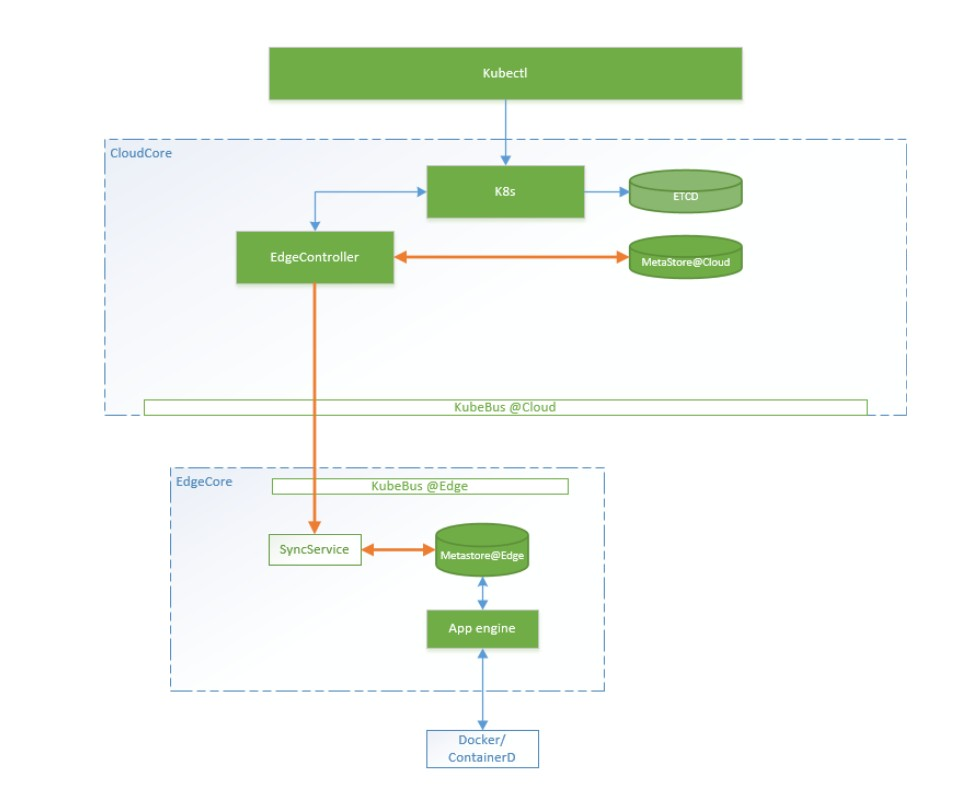
\includegraphics[width=0.5\textwidth]{resources/chapter-2/arsitektur-kube-edge.jpg}
  \caption{Arsitektur KubeEdge \parencite{kubeedge}}
  \label{fig:arsitektur-kube-edge}
\end{figure}

\subsection{Microk8s}
MicroK8s adalah sebuah platform \textit{open-source} yang digunakan untuk mengotomatisasi distribusi, \textit{scaling}, dan manajemen aplikasi yang berbasis kontainer. MicroK8s menyediakan fungsionalitas inti pada Kubernetes, dengan ukuran yang kecil, dan dapat di-\textit{scale} dari satu node hingga menjadi kluster produksi yang besar \parencite{microk8s}.

Dengan mengurangi penggunaan sumber daya yang dibutuhkan untuk menjalankan Kubernetes, MicroK8s memungkinkan penggunaan Kubernetes dalam berbagai lingkungan, seperti:

\begin{enumerate}
  \item Mengubah Kubernetes menjadi alat pengembangan yang ringan.
  \item Menjadikan Kubernetes tersedia untuk digunakan dalam lingkungan minimal seperti GitHub CI (Continuous Integration).
  \item Menyesuaikan Kubernetes untuk aplikasi IoT pada perangkat dengan sumber daya terbatas.
\end{enumerate}


\subsection{K3s}
K3s adalah sebuah platform \textit{open-source} yang memfasilitasi penggunaan Kubernetes dengan ukuran yang lebih ringan dan mudah diimplementasikan. K3s dikembangkan untuk memudahkan distribusi dan manajemen Kubernetes dalam lingkungan yang lebih sederhana dan bersifat minimalis. K3s dibuat untuk mendukung pengembangan pada ranah IoT karena K3s memiliki dukungan sepenuhnya untuk arsitektur ARM serta cocok untuk digunakan pada lingkungan \textit{edge} dan IoT \parencite{k3s}.

K3s memiliki dua komponen utama, yaitu \textit{server} dan \textit{agent}. \textit{Server} dapat dikatakan sebagai sebuah \textit{control plane} atau \textit{master node} yang digunakan pada K3s dan berfungsi untuk mengatur seluruh permintaan ataupun \textit{request} dari \textit{agent}. \textit{Server} memiliki tanggung jawab penuh terhadap masing masing \textit{agent} yang terhubung mulai dari menyimpan data dari masing masing \textit{agent}, \textit{controller}, serta \textit{scheduler} \parencite{k3s}. Di sisi lain, \textit{agent} berfungsi sebagai \textit{slave node} yang akan mengeksekusi semua perintah dari \textit{server} atau \textit{master node}. Ilustrasi arsitektur dapat dilihat pada gambar \ref{fig:arsitektur-k3s}.

\begin{figure}[ht]
  \centering
  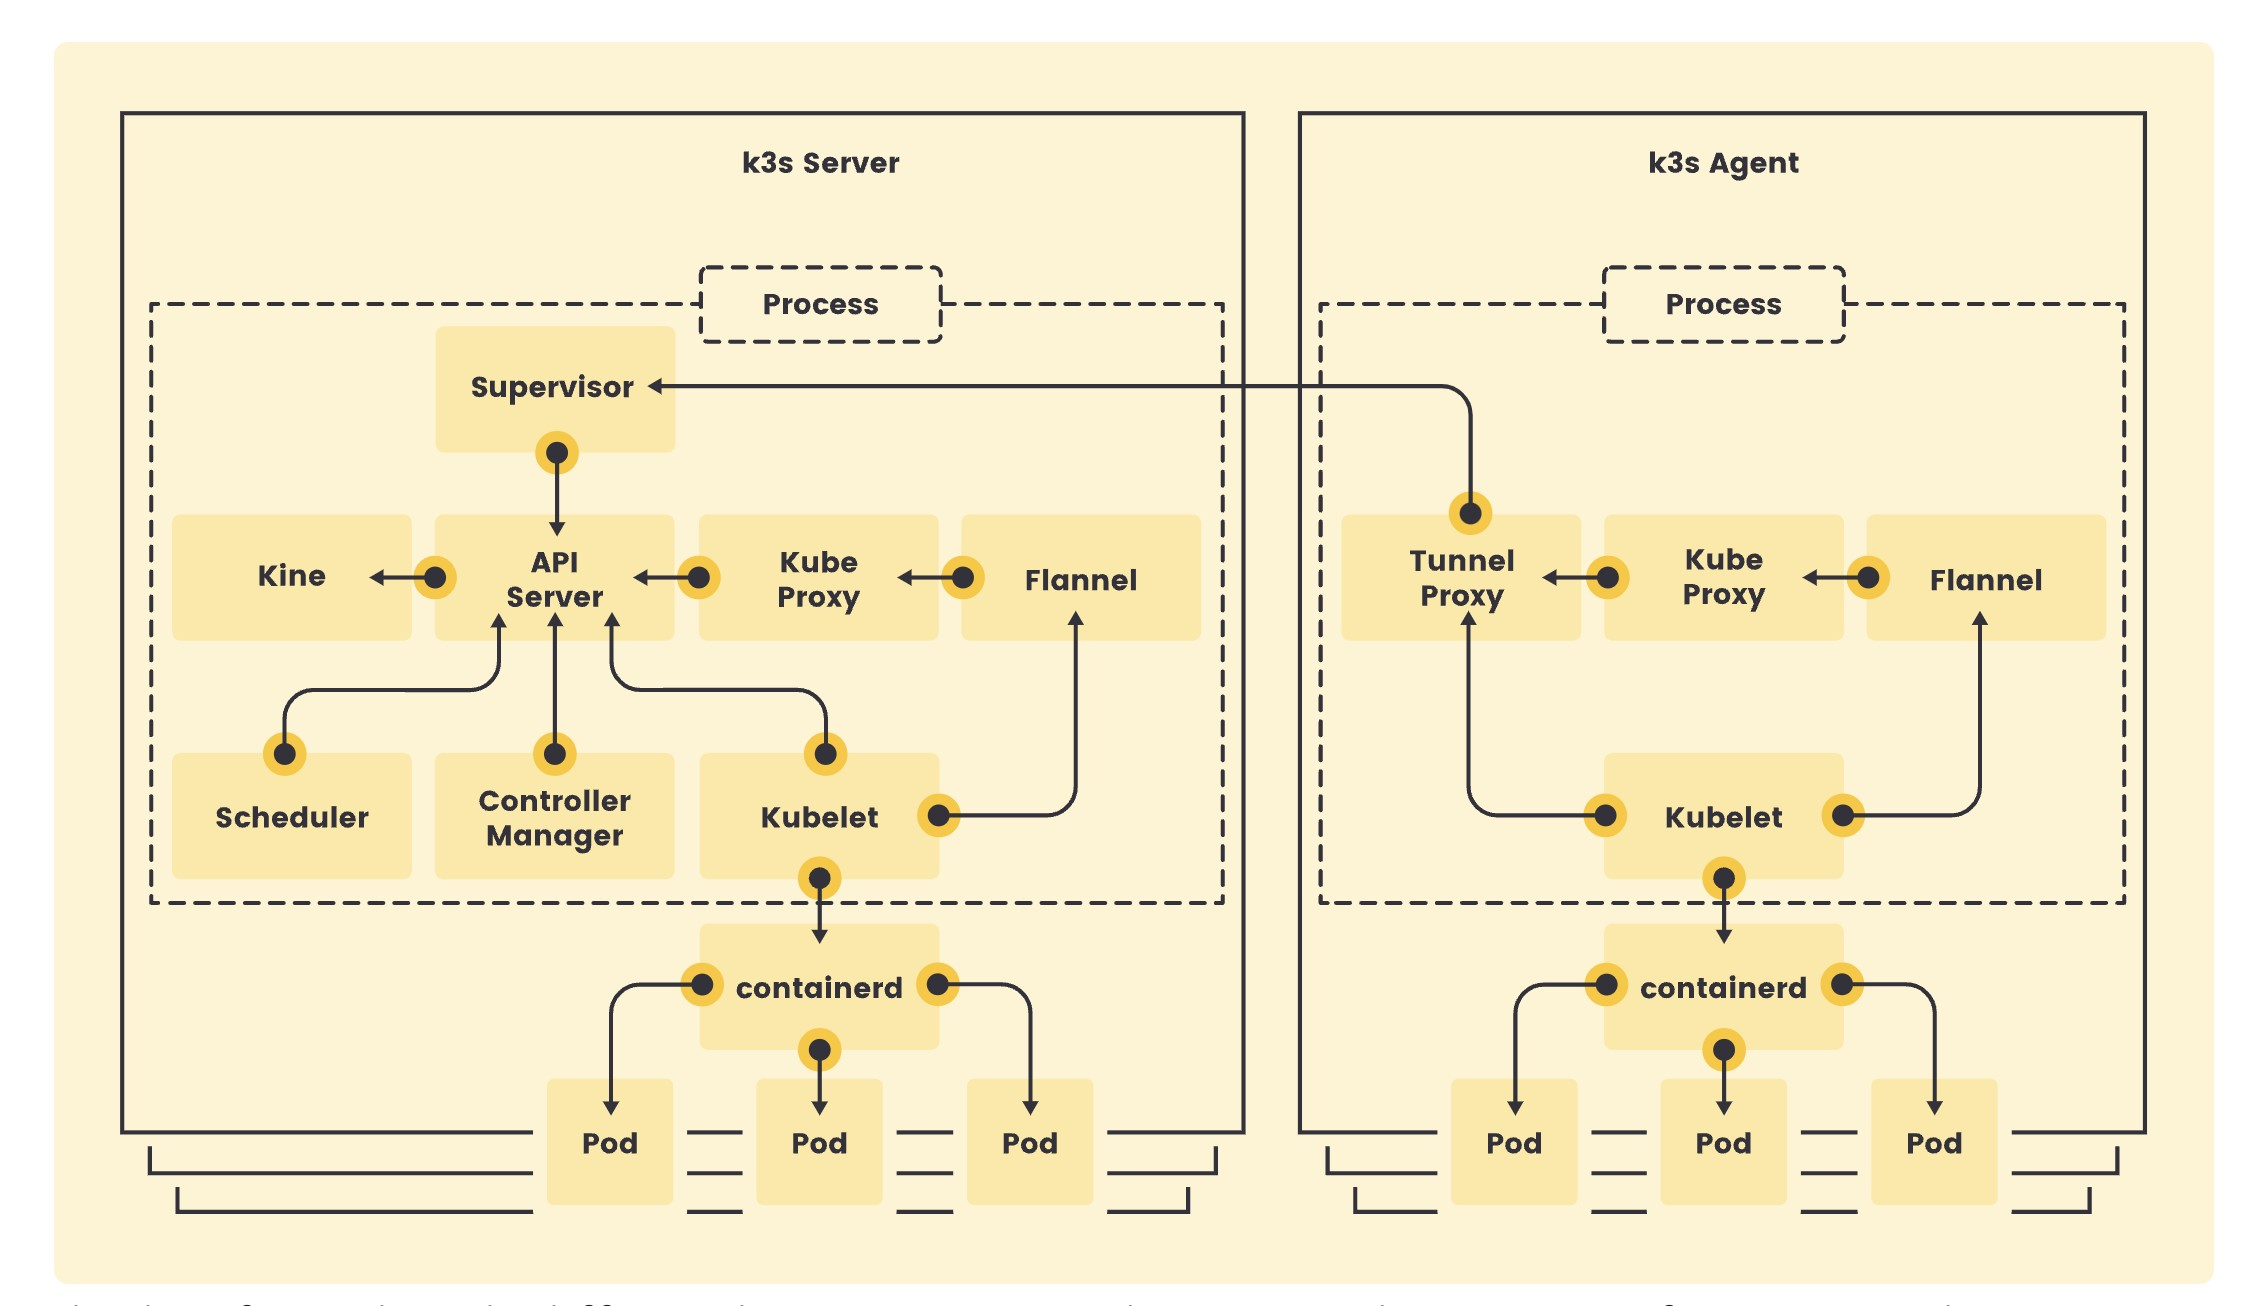
\includegraphics[width=1\textwidth]{resources/chapter-2/arsitektur-k3s.jpg}
  \caption{Arsitektur K3s \parencite{k3s}}
  \label{fig:arsitektur-k3s}
\end{figure}

\pagebreak

\section{\textit{IoT}}

\textit{Internet of Things (IoT)} adalah paradigma teknologi yang mengintegrasikan objek fisik dengan sensor, perangkat keras, dan teknologi jaringan, memungkinkan objek-objek ini untuk mengumpulkan dan bertukar data secara \textit{real-time}. Konsep ini merupakan perwujudan dari evolusi teknologi informasi, di mana objek sehari-hari bertransformasi menjadi entitas cerdas yang mampu berinteraksi dengan lingkungan sekitarnya dan jaringan digital secara lebih luas. \textit{IoT} memperkenalkan kemungkinan baru dalam otomatisasi dan pengambilan keputusan yang berbasis data, membuka jalan bagi inovasi lintas sektor \parencite{madakam2015internet}.

\begin{figure}[ht]
  \centering
  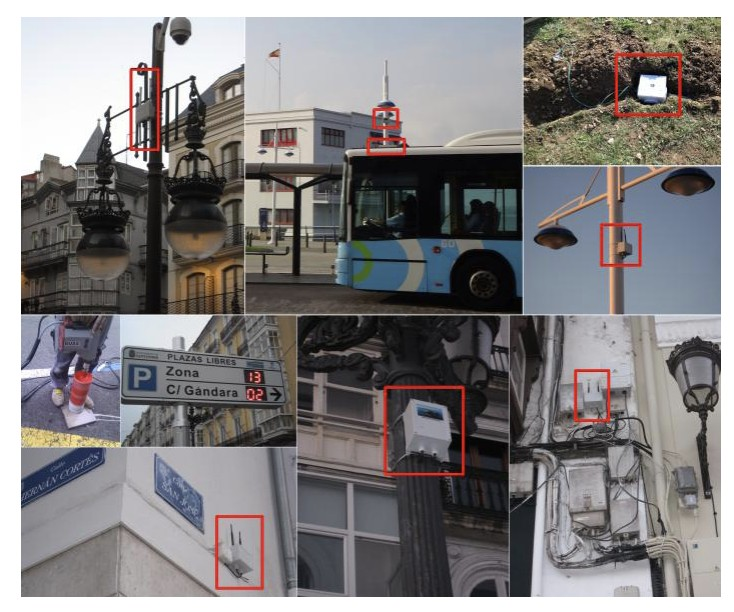
\includegraphics[width=0.8\textwidth]{resources/chapter-2/gambar-iot.jpg}
  \caption{Perangkat IoT yang Terdapat pada Lingkungan Sekitar \parencite{sotres2017practical}}
  \label{fig:iot-kehidupan-sehari-hari}
\end{figure}

\textit{IoT} memiliki aplikasi yang luas di berbagai sektor, termasuk industri, kesehatan, transportasi, dan pertanian. Dalam sektor industri, \textit{IoT} memungkinkan otomatisasi proses dan pemantauan efisiensi mesin secara real-time. Di bidang kesehatan, \textit{IoT} berkontribusi pada pengembangan perangkat medis yang terhubung untuk pemantauan kesehatan pasien. Dalam transportasi, \textit{IoT} mendukung pengembangan kendaraan otonom dan sistem manajemen lalu lintas cerdas. Di sektor pertanian, \textit{IoT} digunakan untuk memantau kondisi tanah dan iklim, membantu petani dalam pengambilan keputusan seperti pada gambar \ref{fig:iot-kehidupan-sehari-hari}

Dalam penerapannya \textit{IoT} dapat dibagi menjadi tiga lapisan, yaitu lapisan persepsi, lapisan jaringan, dan lapisan aplikasi secara berurutan. Lapisan persepsi bertanggung jawab atas pengumpulan data dalam \textit{IoT}. Lapisan ini terdiri dari berbagai jenis sensor, seperti sensor suhu, sensor kelembaban, RFID, kamera, GPS, dan sebagainya. Lapisan jaringan terdiri dari berbagai jenis jaringan, seperti internet, jaringan komunikasi 2G dan 3G, serta jaringan siaran. Lapisan jaringan terutama digunakan untuk mengumpulkan data dari lapisan persepsi dan memproses data tersebut untuk lapisan aplikasi. Terakhir yaitu Lapisan aplikasi, Lapisan ini adalah antarmuka antara pengguna dan \textit{IoT}. Banyak aplikasi, termasuk logistik, rantai pasokan, pertanian, industri, keamanan publik, pengelolaan perkotaan, telemedis, rumah pintar, transportasi pintar, dan pemantauan lingkungan, diaktifkan melalui \textit{IoT} \parencite{SmartHomeSystemBasedOnIoTTechnologies}.

Seiring bertambahnya jumlah perangkat \textit{IoT} perlu dibuat suatu cara agar sistem \textit{scalable}. \textit{Device discovery} merupakan salah satu masalah yang perlu diatasi untuk membuat sistem \textit{IoT} yang \textit{scalable} karena dapat meningkatkan \textit{quality of service} sehingga meningkatkan availabilty \parencite{DeviceDiscovery}. Tidak hanya itu, banyak munculnya perangkat \textit{IoT} baru yang memerlukan \textit{update} secara berkala menimbulkan masalah baru yaitu sulitnya untuk melakukan \textit{update} untuk setiap perangkat yang ada apabila jumlahnya semakin meningkat sehingga peran \textit{remote deployment} menjadi sangat penting dalam menyelesaikan masalah ini \parencite{RemoteDeployment}.

\section{\textit{Smart Home System}}

\textit{Smart home system} adalah integrasi dari tekonologi dan layanan melalui jaringan rumah untuk menciptakan kehidupan yang lebih \textit{seamless}. \textit{Smart home system} menggunakan berbagai macam teknologi untuk melakukan control dan monitor segala perangkat dan interaksinya yang berada pada lingkungan rumah. \textit{Smart home system} bertujuan untuk menciptakan lingkungan yang efisien, aman, serta memudahkan pekerjaan harian yang redundan sehingga hal seperti ini dapat diotomasi dengan mudah \parencite{kadam2015smart}.



\section{Penelitian dan Riset Terkait}
\label{sec:riset-terkait}
Berikut adalah beberapa penelitian dan riset yang pernah dilakukan sebelumnya dan berhubungan dengan tugas akhir ini.

\subsection{LEONORE, \textit{Large-Scale Provisioning of
    Resource Constrained
    IoT Deployments}}
Riset dilakukan oleh Michael Vogler, Johannes M. Schleicher, Christian Inzinger, Stefan Nastic, Sanjin Sehic and Schahram Dustdar dari Vienna University of Technology. Riset ini menjelaskan mengenai cara pembuatan sebuah infrastruktur untuk melakukan \textit{provisioning} perangkat \textit{IoT} dalam skala besar.

\subsection{China Electronic Toll Colleciton}
China memiliki masyarakat yang sangat banyak dan setiap masyarakat memiliki sekurang kurangnya satu kendaraan. Seiring bertambah nya masyarakat di China, maka jalanan yang ada di China akan semakin penuh dengan kendaraan yang akan menghasilkan kemacetan terutama pada tol bagian pembayaran. Untuk mengatasi masalah ini China menggunakan \textit{Electronic Toll Colleciton (ETC)} yang di integrasikan dengan setiap kendaraan untuk mempercepat proses ini \parencite{penelitianterkait1}.

China menggunakan KubeEdge untuk melakukan proses \textit{deployment} \textit{ETC} untuk 100,000 \textit{nodes} dengan total 500,000 aplikasi yang diluncurkan menggunakan KubeEdge tersebar untuk 29 dari 34 provinsi. Proses \textit{deployment} dilakukan secara otomatis dengan membuat sistem \textit{workflow engine} pada kubernetes sehingga proses \textit{deployment} dapat dilakukan dengan cepat dan mudah. Dengan menggunakan metode ini sistem pembayaran tol di China menjadi 10x lebih cepat dari sebelumnya \parencite{penelitianterkait1}.

\begin{figure}[ht]
  \centering
  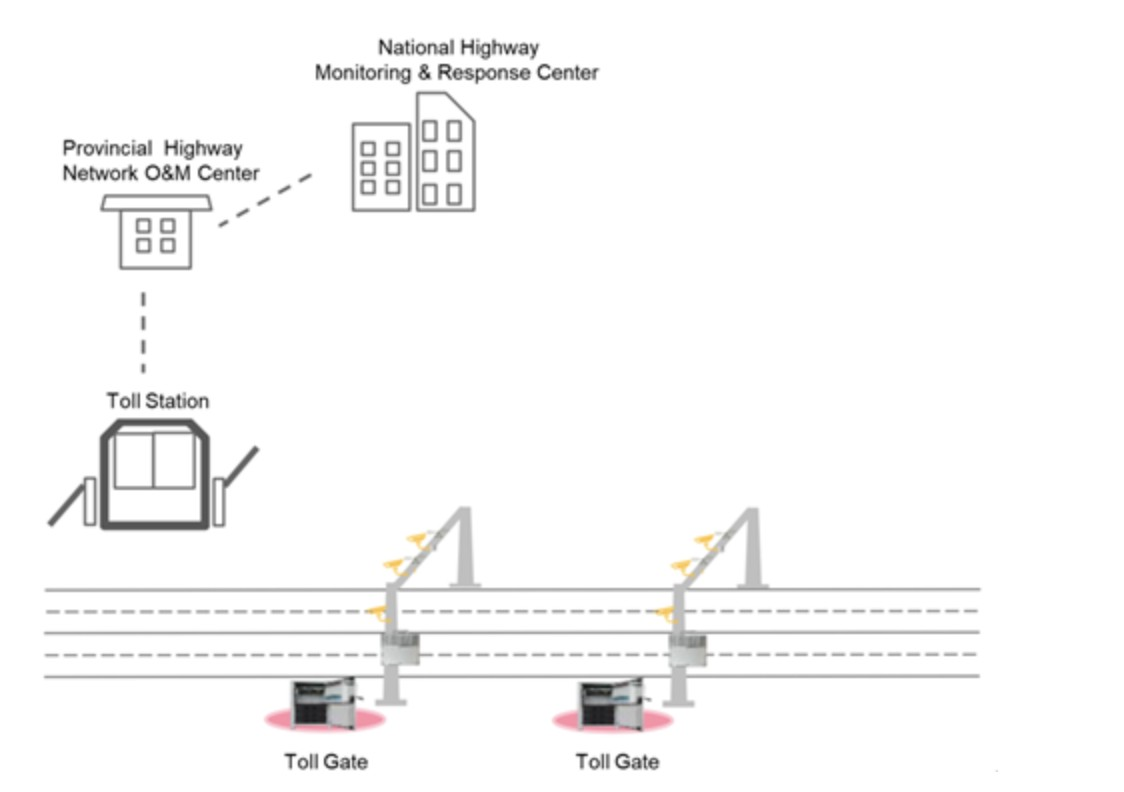
\includegraphics[width=0.8\textwidth]{resources/chapter-2/china-highways.jpg}
  \caption{Implementasi Sistem \textit{ETC} di China \parencite{penelitianterkait1}}
  \label{fig:china-highways}
\end{figure}

\begin{figure}[ht]
  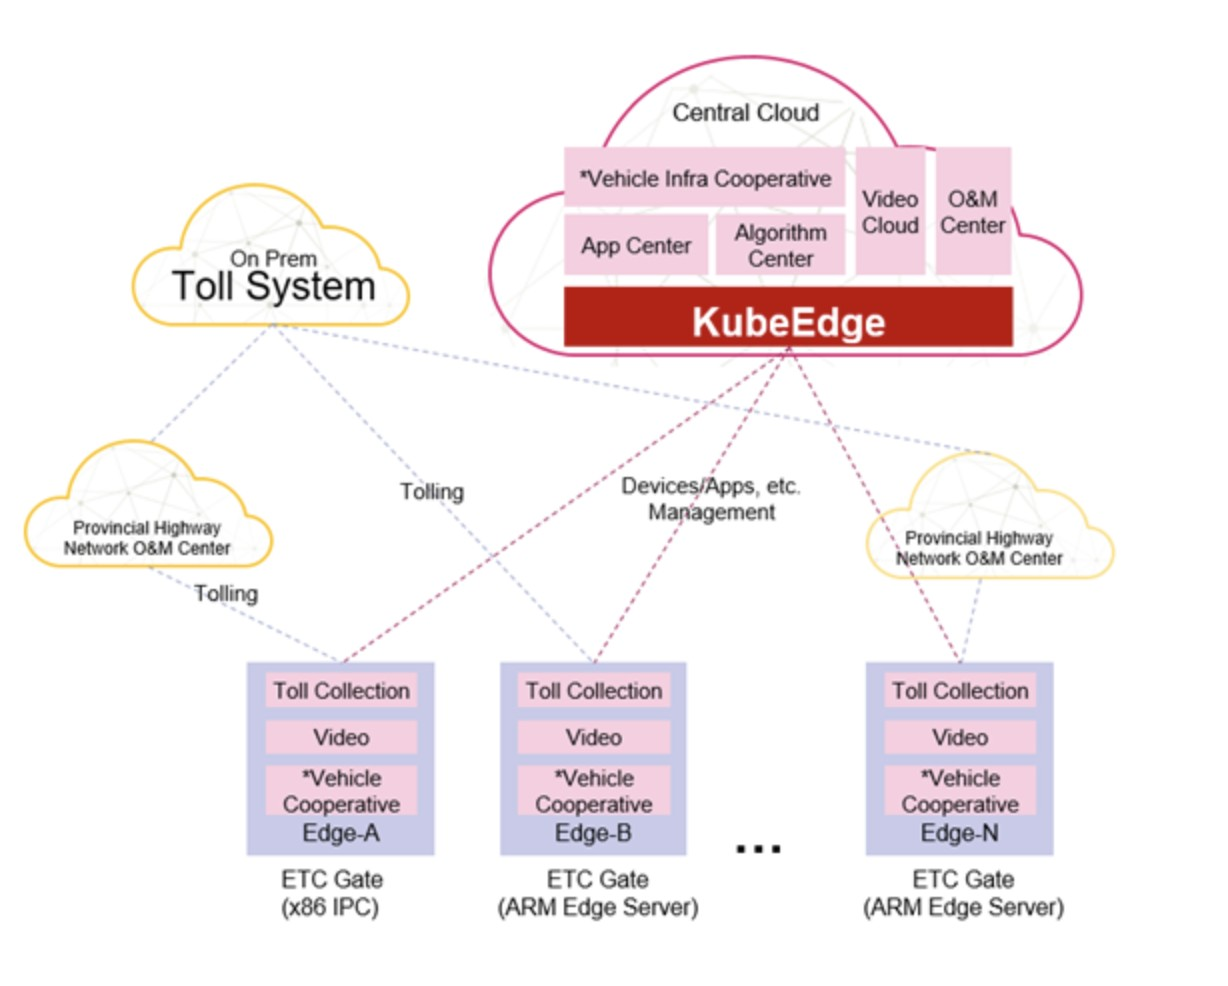
\includegraphics[width=0.8\textwidth]{resources/chapter-2/arsitektur-china-highways.jpg}
  \caption{Arsitektur Sistem \textit{ETC} di China \parencite{penelitianterkait1}}
  \label{fig:architecture-china-highways}
\end{figure}
\subsection{A Model for the Remote Deployment, Update, and Safe Recovery for Commercial Sensor-Based IoT Systems}
Penelitian ini menggali tantangan-tantangan khusus terkait infrastruktur yang didedikasikan untuk penyebaran dan manajemen aplikasi secara jarak jauh. Penelitian ini membahas tantangan-tantangan manajemen terkait sistem sensor IoT dan mengusulkan sebuah cara serta metodologi untuk mengatasi hal tersebut.

Penelitian ini mengimplementasikan solusi sebagai sistem infrastruktur perangkat lunak untuk produk IoT bisnis yang lengkap. Penelitian ini melakukan \textit{deployment} pada 100 perangkat penjual minuman yang tersebar di tiga lokasi. Setiap perangkat bergantung pada sensor yang memantau statusnya dan pada \textit{gateway} yang mengendalikan perilakunya. Arsitektur sistem dapat dilihat pada gambar \ref{fig:architecture-remote-deployments}.

\begin{figure}[ht]
  \centering
  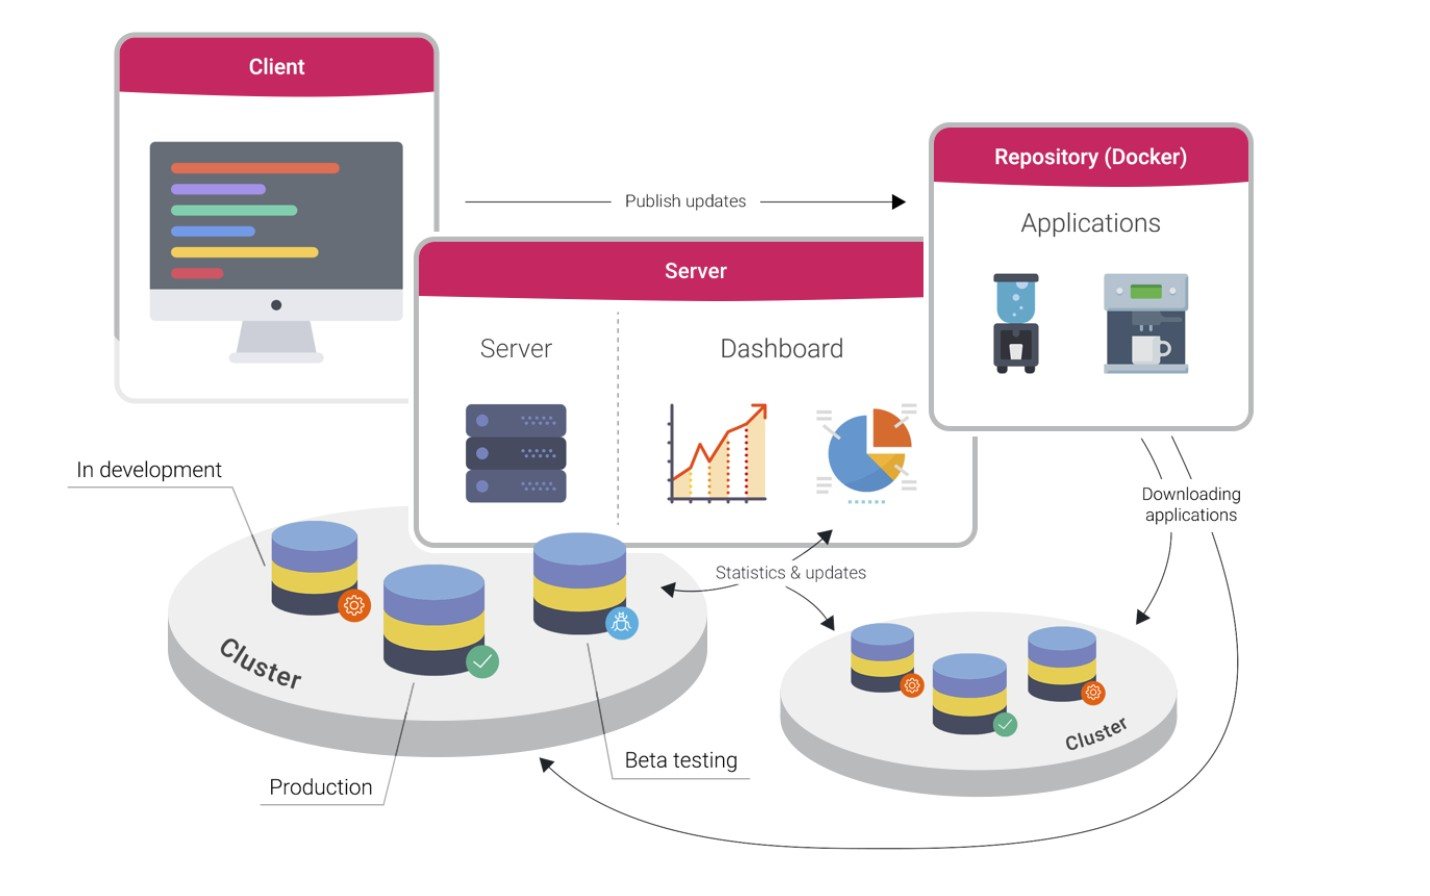
\includegraphics[width=0.8\textwidth]{resources/chapter-2/arsitektur-remote-deployment.jpg}
  \caption{Arsitektur Remote \textit{Deployment} \parencite{RemoteDeployment}}
  \label{fig:architecture-remote-deployments}
\end{figure}

Selama penelitian ini berlangsung, penelitian ini berhasil menerima 133 \textit{update} pada perangkat IoT. 80\% perangkat beroperasi tanpa gangguan selama 250 hari. Sedangkan, 20\% mengalami kegagalan akibat faktor eksternal. Dari 80\% tersebut, 30\% mengalami kegagalan pembaruan sementara akibat kapabilitas perangkat yang berkurang \parencite{RemoteDeployment}.

Solusi yang dibuat penelitian ini mengandalkan keamanan serta \textit{failsafe} yang dapat melakukan \textit{remote deployment} dengan baik serta aman sehingga dapat mendeteksi kegagalan yang terjadi pada perangkat dan melakukan \textit{recovery} dengan cepat. Berikut merupakan beberapa cara untuk melakukan \textit{remote deployment} atau seringkali disebut sebagai OTA \textit{(Over the air)}.

\begin{figure}[ht]
  \centering
  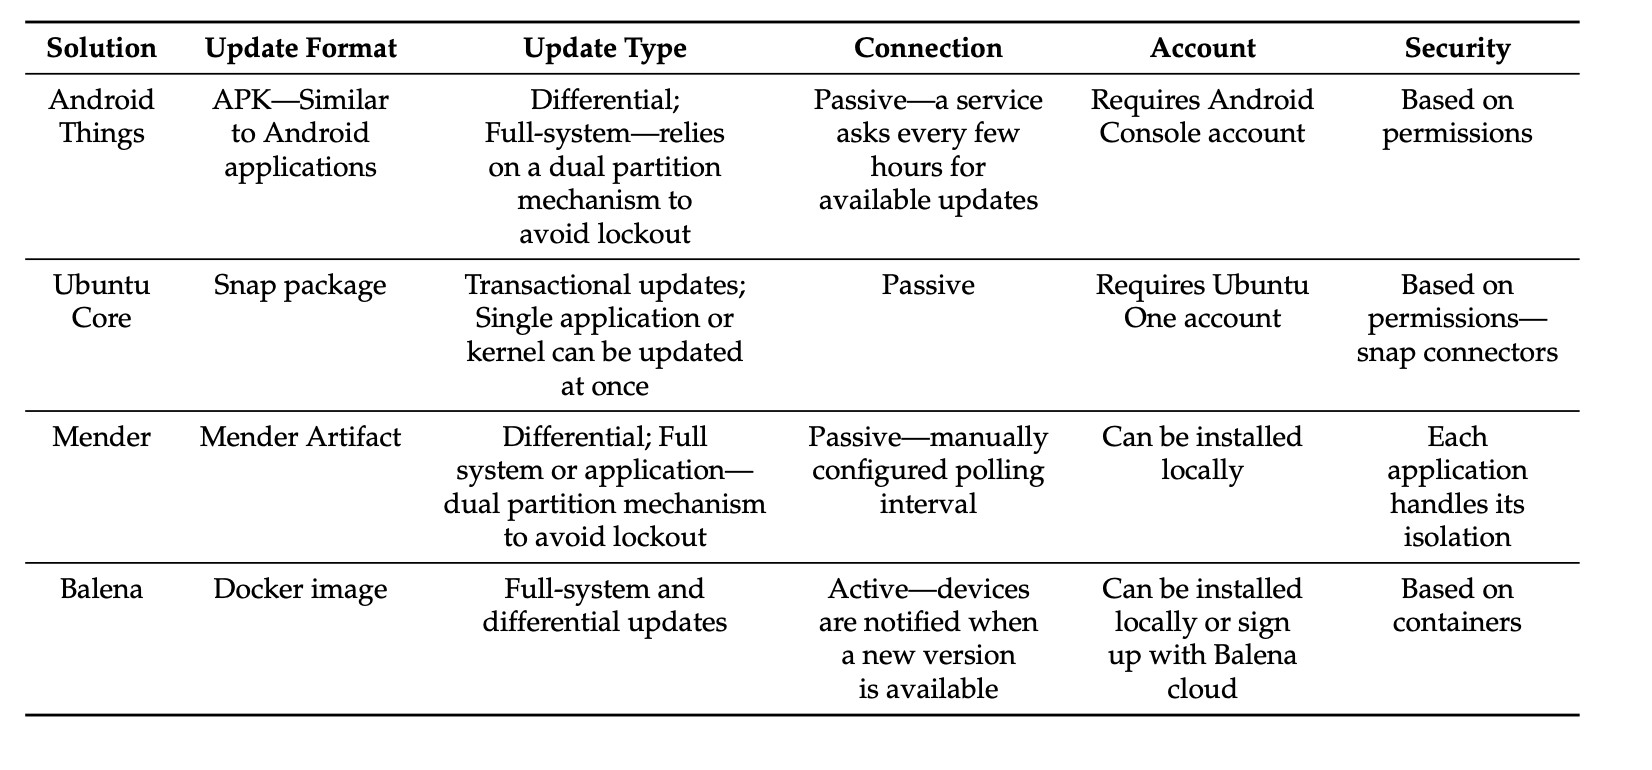
\includegraphics[width=0.8\textwidth]{resources/chapter-2/perbandingan-remote-deployment.jpg}
  \caption{Perbandingan Tata Cara \textit{Remote Deployment} \parencite{RemoteDeployment}}
  \label{fig:comparison-remote-deployments}
\end{figure}

Dapat dilihat dari gambar \ref{fig:comparison-remote-deployments} bahwa terdapat berbagai solusi untuk berbagai tipe \textit{remote deployment}. Pada kasus ini, dapat dibuat suatu cara yang mengadopsi \textit{update type} serta koneksi dari keempat tipe tersebut. Perangkat melakukan \textit{polling} kepada \textit{server} untuk mengecek apakah terdapat versi terbaru atau tidak. Selain itu, dari sisi \textit{Server} juga dapat membuat suatu notifikasi yang dapat diterima oleh perangkat jika terdapat \textit{update} baru yang siap digunakan.



% \section{\textit{Inverted Index}}
\label{sec:invertedindex}

\textit{Inverted Index} merupakan struktur data yang biasa digunakan untuk mesin pencari \parencite{invertedindex2}. Tujuan dari implementasi struktur data ini pada mesin pencari adalah untuk mengoptimalkan kecepatan query dalam mencari dokumen yang mengandung kata kunci tertentu. Struktur data ini melakukan pemetaan terhadap kata dan kumpulan tupel yang berisikan \textit{identifier} (ID) dokumen dan posisi karakter \parencite{invertedindex}. Struktur data ini biasanya dipakai untuk menggantikan \textit{Forward Index}. \textit{Forward Index} adalah struktur data yang menyimpan seluruh kata dalam sebuah dokumen sehingga jika \textit{forward index} di-\textit{query}, maka akan memerlukan iterasi sekuensial pada setiap dokumen dan kata kunci untuk membuktikan dokumen relevan. Sumber daya waktu, memori, dan pemrosesan yang dibutuhkan untuk melakukan query semacam itu tidak realistis dan praktis karena nyatanya, mesin pencari harus melakukan hal tersebut ke ratusan hinga jutaan dokumen. Dengan inverted index yang dibuat, query dapat diselesaikan dengan cara langsung melompat ke \textit{identifier} (ID) kata kunci melalui \textit{random access} pada inverted index untuk mendapatkan \textit{identifier} (ID) dokumen dan posisi karakter.

% \section{\textit{Elastic Search}}
% \textit{Elastic Search} adalah aplikasi mesin pencarian RESTful.  \textit{Elastic Search} diciptakan sebagai pembungkus dan inovasi dari Apache Lucene yang sekedar hanya \textit{library} karena aplikasi yang beredar saat ini tidak hanya dibuat di atas Java dan membutuhkan fleksibilitas yang tinggi, sedangkan, Apache Lucene terkenal sangat sulit untuk orang awam yang tidak memahami istilah-istilah dan \textit{information retrieval}. \textit{Elastic Search} sendiri dibuat menggunakan Java namun menggunakan \textit{Application Programming Interface} RESTful melalui protokol HTTP sehingga aplikasi dengan bahasa apapun dapat dengan mudah menggunakan aplikasi ini. Tidak hanya itu, API dari \textit{Elastic Search} ini juga sudah sangat dipermudah sehingga pemakai tidak perlu mengetahui istilah-istilah dalam Apache Lucene. Sehingga, \textit{Elastic Search} ini sangat dekat dengan proses umum pada data seperti menyimpan, membaharui, menghapus, pengindeksan, pencarian, dan sebagainya.

\textit{Elastic Search} merupakan sebuah perangkat lunak \textit{open-source} yang ditulis menggunakan bahasa pemrograman Java. \textit{Elastic Search} dibangun di atas Apache Lucene. \textit{Elastic Search} menyimpan data secara terpusat untuk pencarian secepat kilat dan relevan \parencite{elasticsearchorigin}. Selain Apache Lucene, \textit{Elastic Search} memanfaatkan teknologi-teknologi lain untuk meningkatkan fungsionalitas dan kinerja, seperti Apache Hadoop untuk big data processing, Apache Spark untuk data analytics, dan Apache Storm untuk real-time stream processing.

\textit{Elastic Search} didesain sebagai sebuah sistem terdistribusi, yang berarti data yang disimpan pada \textit{Elastic Search} akan didistribusikan ke beberapa \textit{node} atau lebih dikenal sebagai \textit{sharding}, sehingga memungkinkan untuk meningkatkan kinerja, skalabilitas, dan ketahanan pada sistem. Sistem terdistribusi pada \textit{Elastic Search} dapat diatur dan dikonfigurasi agar dapat dijalankan pada beberapa \textit{node} yang terpisah atau pada \textit{cluster} yang terhubung, yang memungkinkan pengguna untuk menyimpan data yang sangat besar dan menjalankan query secara paralel pada beberapa node pada waktu yang bersamaan.

\textit{Elastic Search} dibuat untuk memudahkan pengguna mengakses data dan melakukan pencarian pada data yang besar dan kompleks dengan cepat dan efisien. Meskipun Apache Lucene telah menyediakan fitur-fitur yang bagus untuk \textit{indexing} dan \textit{searching}, tetapi Apache Lucene lebih fokus pada teknologi inti dan pengembangan secara \textit{information retrieval} seperti mengoptimisasi dan pengembangan \textit{indexing} dan \textit{searching}. Hal tersebut menyebabkan penggunaan Lucene memerlukan banyak pengaturan dan konfigurasi tambahan untuk bisa diintegrasikan dengan aplikasi yang lebih besar. Dalam hal ini, \textit{Elastic Search} hadir sebagai sebuah solusi yang lebih terintegrasi, mudah digunakan, dan dapat diatur secara fleksibel. \textit{Elastic Search} memanfaatkan Lucene sebagai mesin pencari, tetapi menambahkan banyak fitur-fitur dan fungsionalitas tambahan untuk meningkatkan kinerja dan kemudahan penggunaan. Selain itu, \textit{Elastic Search} dirancang sebagai aplikasi dengan sistem terdistribusi dan \textit{scalable} yang memungkinkan data terdistribusi di beberapa node atau \textit{sharding}, sehingga memungkinkan \textit{Elastic Search} untuk mengatasi masalah data yang sangat besar dan kompleks secara efektif dan efisien. Sedangkan, Lucene hanya pada batas kakas atau \textit{library}.

\textit{Elastic Search} dapat digunakan dengan protokol HTTP dan REST API. Dalam penggunaan dengan protokol HTTP, \textit{Elastic Search} menyediakan endpoint API RESTful HTTP yang dapat diakses oleh pengguna dengan memakai klien HTTP, seperti perintah cURL, \textit{Postman} atau \textit{web browser}. Pengguna dapat membuat permintaan HTTP seperti GET, POST, PUT, DELETE ke API endpoint melalui klien HTTP, dan \textit{Elastic Search} akan memberikan respon sesuai dengan permintaan.

Dalam \textit{Elastic Search} terdapat beberapa operasi yang dapat dilakukan, diantaranya:
\begin{enumerate}
    \item \textbf{\textit{Index}}
    
    Operasi ini akan dijelaskan secara khusus pada bagian selanjutnya, \ref{sec:index}.

    \item \textbf{\textit{Get}}
    
    Operasi \textit{Get} digunakan untuk mengambil dokumen individual berdasarkan ID-nya dari indeks tertentu.
    
    \item \textbf{\textit{Query}}
    
    \textit{Query} digunakan untuk melakukan pencarian dan pengambilan data yang sesuai dengan kriteria tertentu. \textit{Elasticsearch} menyediakan berbagai jenis query seperti pencarian teks lengkap, pencocokan kata kunci, pencocokan frasa, pencarian fuzzy, dan lain-lain.
    
    \item \textbf{\textit{Fetch}}
    
    \textit{Fetch} adalah proses pengambilan dokumen lengkap dari indeks setelah melakukan query. Saat ditemukan, \textit{Elasticsearch} mengambil dokumen dari indeks dan akan digunakan sebagai respon kepada pengguna.
    
    \item \textbf{\textit{Scroll}}
    
    \textit{Scroll} adalah mekanisme pengambilan dokumen yang banyak dari hasil pencarian tanpa perlu mengirimkan \textit{query} ulang. Hal ini menyebabkan pengambilan dokumen dapat menjadi lebih efisien dalam beberapa permintaan, namun, dalam beberapa kasus, bisa menjadi lebih lama untuk mengambil semua dokumen yang relevan.
    
    \item \textbf{\textit{Suggest}}
    
    \textit{Suggest} adalah mekanisme untuk memberikan saran atau \textit{autocompletion} saat pengguna memasukkan kata kunci atau frasa. Biasanya digunakan untuk \textit{autocompletion}, pengoreksi kesalahan pengejaan, dan saran pencarian lainnya.
    
    \item \textbf{\textit{Bulk}}
    
    \textit{Bulk} adalah operasi yang digunakan untuk memasukkan atau memperbarui beberapa dokumen dalam satu permintaan.
    
    \item \textbf{\textit{Flush}}
    
    \textit{Flush} adalah operasi yang digunakan untuk mengosongkan memori \textit{cache} dan menulis data yang tertunda ke disk. Operasi ini memastikan bahwa data yang ditulis telah disimpan secara permanen di indeks.
    
    \item \textbf{\textit{Refresh}}
    
    \textit{Refresh} adalah operasi yang digunakan untuk membuat perubahan yang terjadi pada indeks secara terlihat dan dapat dicari. Saat melakukan operasi indeks seperti menambahkan atau menghapus dokumen, perubahan tersebut tidak langsung terlihat oleh pencarian hingga dilakukan operasi refresh.
\end{enumerate}

% \section{Java \textit{Virtual Machine}}
\textit{Java Virtual Machine} atau JVM adalah program yang dapat membaca program java yang telah dikompilasi atau biasa dikenal sebagai \textit{java bytecode} dan menginterpretasikannya menjadi bahasa mesin yang dapat dieksekusi oleh komputer \parencite{java12}. Secara tidak langsung, JVM merupakan komponen utama dalam menjalankan program bahasa Java. Struktur JVM terdiri dari \textit{runtime data structure} di memori dan dua subsistem yang berhubungan langsung dengan \textit{runtime data structure} yaitu \textit{class loader} dan \textit{execution engine}. Semua program yang dibuat dengan Java akan dikompilasi ke \textit{java bytecode} yang nantinya akan diinterpretasikan oleh JVM untuk dieksekusi komputer.

\textit{Elastic Search}, yang terbuat dari bahasa Java, berjalan di atas platform Java Virtual Machine (JVM). JVM sendiri akan bertanggung jawab untuk menjalankan kode Java dan mengelola sumber daya yang dibutuhkan oleh program, seperti memori, prosesor, dan jaringan. Sehingga, JVM memiliki peran penting dalam menjalankan \textit{Elastic Search} dan memastikan kinerjanya baik. JVM menyediakan opsi pengaturan yang membuat pengguna dapat mengontrol alokasi memori dan penggunaan CPU pada aplikasi \textit{Elastic Search}. Dengan mengatur parameter JVM yang tepat, pengguna dapat memperbaiki kinerja \textit{Elastic Search} dan memaksimalkan penggunaan sumber daya sistem.

Parameter yang berhubungan erat dengan alokasi sumber daya pada \textit{Elastic Search} dan mempengaruhi kinerja JVM adalah parameter \textit{heap size} (-Xms dan -Xmx) yang mengatur ukuran \textit{heap memory} yang dialokasikan untuk JVM. \textit{Heap memory} adalah tempat JVM menyimpan objek dan data dari aplikasi Java yang sedang berjalan. Parameter -Xms menentukan ukuran \textit{heap memory} awal yang dialokasikan ketika JVM dimulai, sedangkan parameter -Xmx menentukan batas maksimal ukuran \textit{heap memory} yang dapat dipakai oleh JVM. Selain itu, terdapat parameter lain yang dapat mempengaruhi kinerja JVM dan \textit{Elastic Search}, seperti \textit{thread pool size}, \textit{circuit breaker settings}, dan lain-lain. Parameter-parameter ini dapat diatur melalui file konfigurasi \textit{Elastic Search} atau melalui command line arguments saat menjalankan \textit{Elastic Search}.

% \section{\textit{Indexing}}
\label{sec:index}

\textit{Indexing} adalah suatu teknik untuk menyusun kata-kata dan mengurangi usaha untuk mencari hal yang berkaitan dengan kata tersebut jika diperlukan, \parencite{database}. Secara umum, indeks banyak digunakan pada buku teks, basis data, dan sistem information retrieval. Seperti salah satu contoh tekniknya adalah \textit{Inverted Index} yang telah dijelaskan pada \ref{sec:invertedindex}.

Terdapat kelebihan penggunaan indeks, diantaranya:
\begin{enumerate}
    \item \textit{Indexing} dapat mempercepat proses pencarian data dengan membuat indeks dan mencocokkan kata kunci dengan indeks tersebut, sehingga mesin dapat menemukan data dengan lebih cepat.
    \item \textit{Indexing} dapat meningkatkan akurasi pencarian dengan menampilkan hasil pencarian yang lebih relevan dengan kata kunci yang dimasukkan.
\end{enumerate}

Namun, ada juga kelemahan dari penggunaan indeks, yaitu sebagai berikut.
\begin{enumerate}
    \item \textit{Indexing} memerlukan ruang penyimpanan tambahan untuk membuat indeks.
    \item Proses pembuatan \textit{indexing} memerlukan waktu, terutama jika data yang akan di-indeks sangat banyak.
\end{enumerate}

Sehingga, dapat disimpulkan penggunaan indeks sangat bermanfaat namun menambahkan biaya.
Pada kasus-kasus dokumen besar, penggunaan indeks pengaruhnya sangat besar karena mesin akan mencari data pada indeks terlebih dahulu sebelum mencari data pada dokumen asli. Hal ini dapat membantu mengurangi waktu pencarian dan menghemat penggunaan memori karena mesin tidak perlu membaca seluruh dokumen untuk menemukan data yang dicari. Namun, apabila \textit{indexing} dilakukan secara berlebihan, akan terdapat banyak indeks yang tidak terpakai dan hanya akan menambah kebutuhan memori.

% Konsep \textit{caching} sendiri adalah menyimpan data yang sering diakses pada level cache atau memori yang lebih dekat dengan CPU agar dapat diakses dengan cepat saat ingin melakukan pencarian, lihat gambar \ref{fig:cache-level}. \textit{Cache} sendiri biasanya memiliki ruang yang terbatas sehingga biasanya membuang data yang sudah tidak diakses sehingga jika dibutuhkan harus dicari ke \textit{storage}. Konsep ini ditiru oleh basis data dan aplikasi \textit{information retrieval} untuk mempercepat proses pencarian dengan memanfaatkan \textit{indexing} untuk mencari (lihat gambar \ref{fig:cache-app}) dan \textit{caching} untuk mengembalikan data yang sering diakses dengan memanfaatkan memori.

% \begin{figure}[h]
%     \centering
%     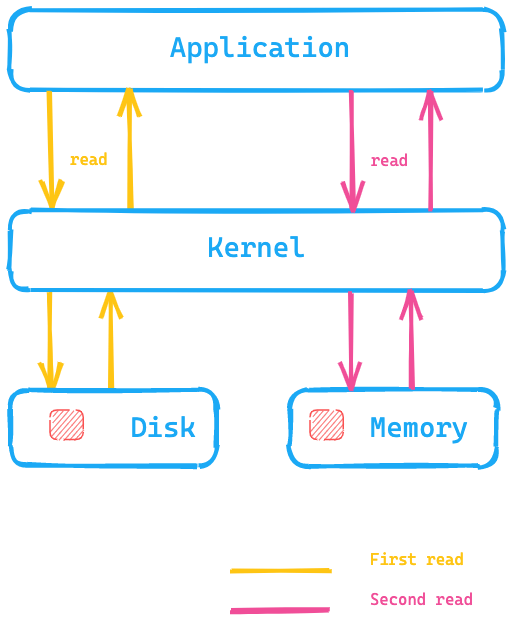
\includegraphics[width=0.5\textwidth]{chapter-2/cache-app.png}
%     \caption{Prinsip Cache pada Aplikasi}
%     \label{fig:cache-app}
% \end{figure}

% \begin{figure}[h]
%     \centering
%     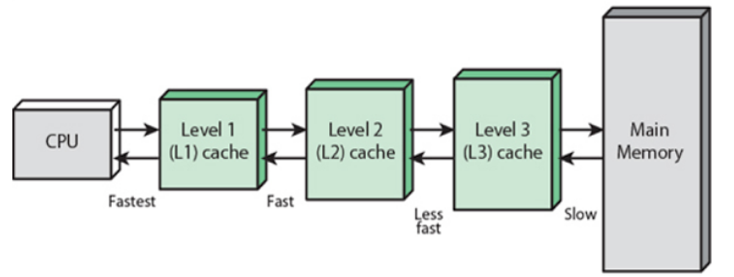
\includegraphics[width=0.5\textwidth]{chapter-2/cache-memory.jpeg}
%     \caption{Level-level pada Cache}
%     \label{fig:cache-level}
% \end{figure}

% \section{\textit{Caching}}
\textit{Caching} adalah teknik menyimpan data atau informasi yang sering digunakan secara lokal pada suatu tempat agar dapat diakses lebih cepat kedepannya. \textit{Caching} dapat digunakan untuk menyimpan hasil pencarian yang sering dilakukan oleh pengguna, sehingga jika pengguna melakukan pencarian yang sama, hasilnya dapat diambil dari \textit{cache} yang tersimpan dan tidak perlu melakukan pencarian.

Terdapat relevansi \textit{caching} dengan indeks, \textit{caching} dapat membantu meningkatkan kinerja sistem indeks dengan menyimpan hasil pencarian yang sering dilakukan dan mengaksesnya dari \textit{cache} saat pengguna melakukan pencarian yang sama. Dengan demikian, waktu dan sumber daya yang diperlukan untuk memproses pencarian dapat dihemat. Pengguna juga dapat mengakses hasil pencarian dengan lebih cepat karena data yang dicari sudah disimpan di \textit{cache} dan tidak perlu memproses ulang dari indeks. Namun, perlu diingat bahwa ukuran cache harus dibatasi, sehingga \textit{caching} tidak menggunakan memori secara berlebihan.

% \input{chapters/chapter-2/15-simulasi}
% \section{Pembelajaran Mesin}
% Pembelajaran Mesin adalah sebuah bidang pembelajaran yang mempelajari pemahaman dan membangun metode untuk "belajar" dengan memanfaatkan data untuk meningkatkan banyak aspek terutama efisiensi dan kualitas terhadap suatu rangkaian tugas. Algoritma pembelajaran mesin membangun model berdasarkan data sampel yang biasa disebut \textit{training data} untuk menghasilkan model yang dapat memprediksi atau membuat keputusan tanpa diprogram secara eksplisit, \parencite{ml}.

% \subsection{\textit{Reinforcement Learning}}
% \textit{Reinforcement learning} atau RL adalah bidang pembelajaran mesin yang mengotomasi sebuah agen untuk mengambil tindakan dan memaksimalkan \textit{reward} dari aksi yang dilakukan, \parencite{reinforcementlearning}. RL adalah salah satu paradigma dari tiga pembelajaran mesin dasar seperti \textit{Supervised Learning} dan \textit{Unsupervised Learning}. Singkatnya, RL membuat agen dapat mengoreksi pengetahuannya secara terus menerus agar dapat memaksimalkan fungsinya. Berbeda dengan \textit{Supervised Learning}, RL tidak memerlukan label dan tidak memerlukan secara eksplisit dikoreksi. Fokus dalam membangun RL, adalah mencari keseimbangan eksplorasi terhadap lingkungan baru dan eksploitasi terhadap pengetahuan yang dimiliki.

% penelitian terkait